\documentclass[border=15pt, multi, tikz]{article}
\usepackage[backend=bibtex,style=authoryear,natbib=true]{biblatex} % Use the bibtex backend with the authoryear citation style (which resembles APA)

\addbibresource{example.bib} % The filename of the bibliography

\usepackage[autostyle=true]{csquotes} % Required to generate language-dependent quotes in the bibliography



\usepackage{amssymb}
\usepackage[backend=bibtex,style=authoryear,natbib=true]{biblatex} % Use the bibtex backend with the authoryear citation style (which resembles \left( APA)

\addbibresource{example.bib} % The filename of the bibliography

\usepackage[autostyle=true]{csquotes} % Required to generate language-dependent quotes in the bibliography
\usepackage{import}
\usepackage{float}
\usepackage{tikz}
\usepackage{tikz-network}
\usepackage{breqn}
\usepackage{bm}
\usepackage{graphicx}
\usepackage{subcaption}
\usepackage{multirow}
\usepackage{pdfpages}
\usepackage{rotating}
\usetikzlibrary{fit}
\usetikzlibrary{calc,patterns,angles,quotes}
\usetikzlibrary {arrows.meta,graphs,shapes.misc}
\usetikzlibrary {positioning}


\usetikzlibrary{fit}
\usetikzlibrary {arrows.meta,graphs,shapes.misc}
\usetikzlibrary {positioning}
\subimport{./layers/}{init}
\newcommand{\bn}{\textbf{n}}
\newcommand{\tabhead}[1]{\textbf{#1}}

\def\ConvColor{rgb:yellow,5;red,2.5;white,5}
\def\ConvReluColor{rgb:yellow,5;red,5;white,5}
\def\PoolColor{rgb:red,1;black,0.3}
\def\DcnvColor{rgb:blue,5;green,2.5;white,5}
\def\SoftmaxColor{rgb:magenta,5;black,7}
\def\SumColor{rgb:blue,5;green,15}
\def\poolsep{1}


\begin{document}

\begin{figure}[th]
	\centering
	
	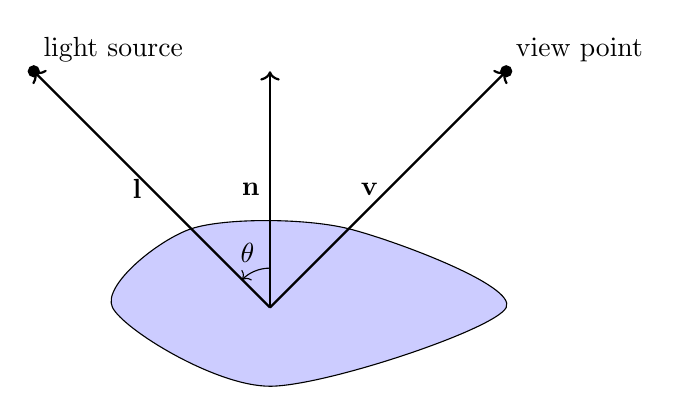
\begin{tikzpicture} 
		% reference lines
		\coordinate (light) at (-1,3);
		\coordinate (p) at (2,0);
		\coordinate (normal) at (2,3);
		\draw [fill=blue!20] plot [smooth cycle] coordinates {(0,0) (1,1) (3,1) (5,0) (2,-1)}; %% surface element
		\draw[thick, ->] (2,0) -- (2,3) node[midway, left] {$ \textbf{n} $}; %% normal
		\draw[thick, ->] (2,0) -- (-1,3) node[midway, left] {$ \textbf{l} $}  ; %% source direction
		\pic [draw, ->, "$\theta$", angle eccentricity=1.5] {angle = normal--p--light};
		\draw[thick, ->] (2,0) -- (5,3) node[midway, left] {$ \textbf{v} $}; %% view direction
		\filldraw[black] (-1,3) circle (2pt) node[anchor=south west]{light source}; %% light source
		\filldraw[black] (5,3) circle (2pt) node[anchor=south west]{view point}; %% view point		
	\end{tikzpicture}
	\caption{The surface normal, source light direction and the view point direction, where $ \theta $ denotes the angle between light direction and the normal.}
	\label{fig:lambertian-surface}
\end{figure}



\end{document}
